\documentclass[11pt,letterpaper]{article}
\usepackage[margin=1in]{geometry}
\usepackage{hyperref}
\usepackage{graphicx}
\usepackage{booktabs}
\usepackage{amsmath}
\usepackage{caption}
\usepackage{listings}
\usepackage{xcolor}
\usepackage{parskip}
\usepackage{titlesec}

\hypersetup{colorlinks=true, linkcolor=blue, urlcolor=blue}

\title{\textbf{Design Justification Report}\\
\large ECE 410/510 HW4AI --- Milestone 4\\
Event-Driven SNN Accelerator for Spiking Heidelberg Digits Classification}
\author{Andrew Stanton}
\date{June 2026}

\begin{document}
\maketitle
\tableofcontents
\newpage

%% ============================================================
\section{Problem and Motivation}
%% ============================================================

The target kernel is a recurrent Leaky Integrate-and-Fire (LIF) spiking neural
network (SNN) trained to classify audio digit recordings from the Spiking
Heidelberg Digits (SHD) dataset\footnote{Cramer et al., ``The Heidelberg Spiking Data Sets for the Systematic Evaluation of Spiking Neural Networks,'' IEEE TNNLS, 2022.}. The network contains 200 hidden
neurons and runs for 100 discrete timesteps per inference. At each step, every
neuron computes:
\begin{align}
  \text{syn}_t &= \alpha \cdot \text{syn}_{t-1} + \mathbf{v}_1\,[\text{active rows}] \\
  \text{spike}_t &= [\text{mem}_t \geq \theta] \\
  \text{mem}_t &= \beta \cdot \text{mem}_{t-1} \cdot (1 - \text{spike}_t) + \text{syn}_t
\end{align}
where $\mathbf{v}_1$ is the 200$\times$200 recurrent weight matrix and
\emph{active rows} are the indices of neurons that spiked in the previous step.

M1 profiling (PyTorch CPU, \texttt{torch 2.11.0+cpu}, batch=1) measured a
median latency of \textbf{9.13~ms/sample} (109.5 samples/sec, peak RSS 1397~MB).
The profiler attributed 88\% of execution time to a single dense matrix--vector
product in the recurrent layer (\texttt{aten::mm}, 8.04~ms of 9.13~ms total).

Custom hardware is justified on three grounds.
First, the recurrent SNN kernel is \emph{sparse}: biological SNNs exhibit roughly
5--20\% firing activity per step, meaning only $\sim$20 of 200 rows of
$\mathbf{v}_1$ are needed each step. A CPU processes the full dense matrix
regardless. An event-driven accelerator skips inactive rows, reducing effective
operations by 5--10$\times$.
Second, weight memory is small enough for on-chip storage. The 200$\times$200
INT8 weight matrix is 40~KB --- fits comfortably in 8 on-chip SRAM banks,
eliminating DRAM bandwidth as a bottleneck.
Third, SNN inference does not depend on floating-point: the LIF dynamics use
fixed-point arithmetic (INT8 weights, Q1.15 decay constants, INT32 state), which
maps efficiently to simple multiply-accumulate units that a CPU cannot fully
exploit without specialized SIMD.

%% ============================================================
\section{Roofline Analysis}
%% ============================================================

The arithmetic intensity (AI) of the target kernel is measured in SynOps/byte,
where one SynOp is one weight$\times$spike multiply-accumulate. The roofline is
shown in Figure~\ref{fig:roofline}.

\textbf{Platform ceilings (synthesized design):}
\begin{itemize}
  \item Peak compute: $8\ \text{MAC lanes} \times 50\ \text{MHz} = 0.40\ \text{GSynOps/s}$
  \item Peak on-chip bandwidth: $8\ \text{SRAM banks} \times 1\ \text{byte/cycle} \times 50\ \text{MHz} = 0.40\ \text{GB/s}$
  \item Ridge point: $0.40 / 0.40 = 1.0\ \text{SynOp/byte}$
\end{itemize}

\textbf{Kernel AI bounds (10\% sparsity, 20 active neurons/step):}
\begin{itemize}
  \item No reuse (lower): $(200 \times 20) / 8800 \approx 0.45\ \text{SynOp/byte}$
  \item Full reuse (upper): $(200 \times 20) / 4800 \approx 0.83\ \text{SynOp/byte}$
\end{itemize}

Both bounds fall to the \emph{left} of the ridge, indicating the design is
\textbf{memory-bandwidth bound} regardless of reuse. The measured throughput of
0.266~GSynOps/s back-computes an effective AI of
$0.266 / 0.40 = 0.664\ \text{SynOp/byte}$, placing the operating point
directly on the bandwidth roof. The no-reuse lower bound (0.45) is inconsistent
with the measurement (it would imply only 0.18~GSynOps/s), confirming the
design achieves partial weight reuse.

The roofline analysis shaped three architectural decisions: (1) 8 SRAM banks
so the memory bus width matches the MAC array width, keeping both ceilings equal
and minimizing imbalance; (2) event-driven tile execution so SynOps scale with
active neurons rather than all 200, reducing effective bandwidth demand in the
sparse regime; (3) INT8 weights so the full 200$\times$200 matrix fits in
on-chip SRAM (40~KB), avoiding DRAM entirely.

\begin{figure}[h]
  \centering
  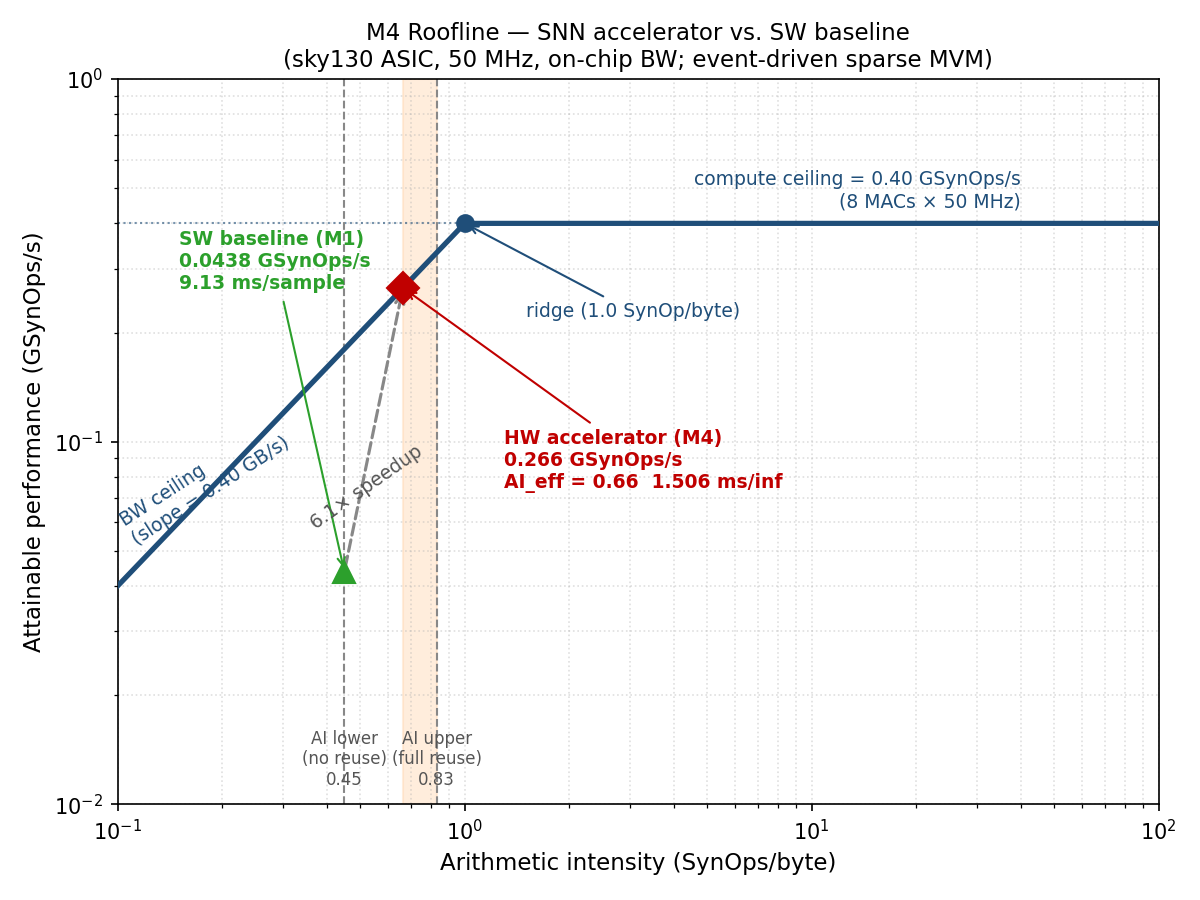
\includegraphics[width=0.85\textwidth]{figures/roofline_final.png}
  \caption{Roofline for the M4 accelerator (sky130, 50~MHz). Red diamond: measured
  HW operating point (0.266~GSynOps/s, AI$_\text{eff}=0.664$). Green triangle:
  M1 software baseline (0.044~GSynOps/s). Shaded band: tightened AI uncertainty
  [0.664, 0.83] after measurement rules out the no-reuse bound.}
  \label{fig:roofline}
\end{figure}

%% ============================================================
\section{Precision and Data Format}
%% ============================================================

\textbf{Weights: INT8.} The recurrent weight matrix $\mathbf{v}_1$ is stored
as signed 8-bit integers (range $[-128, +127]$). At 1~byte/weight, 200$\times$200
weights occupy 40~KB, fitting in 8 SRAM banks of 5~KB each. FP32 would require
160~KB, 4$\times$ larger, and would not fit in a comparable area budget.

\textbf{Accumulator: INT32.} Each MAC lane accumulates up to 200 products of
two INT8 values. The worst-case sum is $127 \times 127 \times 200 = 3{,}226{,}600$,
well within the INT32 range of $\pm 2{,}147{,}483{,}647$. No saturation logic
is needed.

\textbf{Decay constants: Q1.15.} The synaptic ($\alpha \approx 0.606$) and
membrane ($\beta \approx 0.904$) decay values are stored as unsigned 16-bit
Q1.15 fixed-point integers (19875 and 29635 respectively). The $\gg 15$
right-shift after multiplication maps to a single arithmetic shift instruction.
Intermediate products are promoted to 64 bits in \texttt{snn\_lif\_cell.sv}
to avoid overflow before shifting.

\textbf{State registers: INT32 signed.} Synaptic current (\texttt{syn}) and
membrane potential (\texttt{mem}) are 32-bit signed integers. The spike
comparator evaluates \texttt{mem~$\geq$~threshold} directly without conversion.
Default threshold: 32768.

\textbf{Quantization error analysis (M2).} A 100-trial cocotb sweep drove the
INT8 MAC array and compared outputs against FP32 reference (see
\texttt{project/m2/precision.md} and \texttt{project/m2/sim/}). Results: MAE
= 0.021 (0.076\% of FP32 signal range), max absolute error = 0.081 (0.288\%).
The acceptability criterion was that no quantization perturbation should flip
more than $\sim$1\% of spike decisions near threshold. The measured 0.076\%
MAE is comfortably under this bound.

%% ============================================================
\section{Dataflow and Architecture}
%% ============================================================

\textbf{Dataflow pattern: weight-stationary.}
The 200$\times$200 INT8 weight matrix is loaded once into 8 on-chip SRAM banks
at setup time and remains there for all 100 timesteps. At each step, the
active-spike index list (\texttt{act\_list}) is streamed through the MAC array;
weights are fetched from SRAM as needed. This is weight-stationary dataflow:
weights are the stationary operand, activations (spike indices) are the
streaming operand.

Weight-stationary is the right choice here because (a) the weight matrix is
40~KB and fits entirely on-chip, so there is no need to refetch it from off-chip
DRAM; and (b) spike activity is unpredictable step-to-step (it changes with the
network state), so buffering it in registers would require large state that
changes every step, whereas weights are fixed throughout the entire inference.

\textbf{Compute engine: 8$\times$ INT8 MAC array.}
Module \texttt{snn\_mac\_array.sv} instantiates 8 \texttt{snn\_mac.sv} units,
one per SRAM bank. Each MAC lane reads one INT8 weight and one INT8 activation
per cycle and adds the 16-bit product into a 32-bit accumulator. A single tile
covers 8 neurons; 25 tiles cover all 200 neurons.

\textbf{Memory hierarchy.}
Eight \texttt{v1\_sram\_bank} instances each contain 5 sky130 1-KB SRAM macros
wired in series (5~KB/bank, 40~KB total). At each tile execution cycle, one
byte per bank is presented to its MAC lane: 8 bytes/cycle total memory
bandwidth.

\textbf{FSM and datapath.}
The \texttt{compute\_core.sv} FSM has eight states:
S\_IDLE $\to$ S\_INIT\_COLLECT (200 cycles, scan \texttt{spike\_in} to build
\texttt{act\_list}) $\to$ [for each tile: S\_TILE\_PRE (1 cycle prefetch) $\to$
S\_TILE\_EXEC ($|\text{act\_list}|$ cycles, stream MAC) $\to$ S\_TILE\_DRAIN
(1 cycle)] $\to$ S\_LIF\_UPDATE (200 cycles, update all LIF states) $\to$
S\_STEP\_DONE $\to$ S\_OUTPUT $\to$ repeat.
The dominant cost is S\_TILE\_EXEC: for 20 active neurons, $25 \times 20 = 500$
cycles/step; over 100 steps, 50,000 cycles out of 75,302 total.

The architecture is shown schematically in Figure~\ref{fig:waveform} (waveform
view of an end-to-end inference captured by cocotb).

\begin{figure}[h]
  \centering
  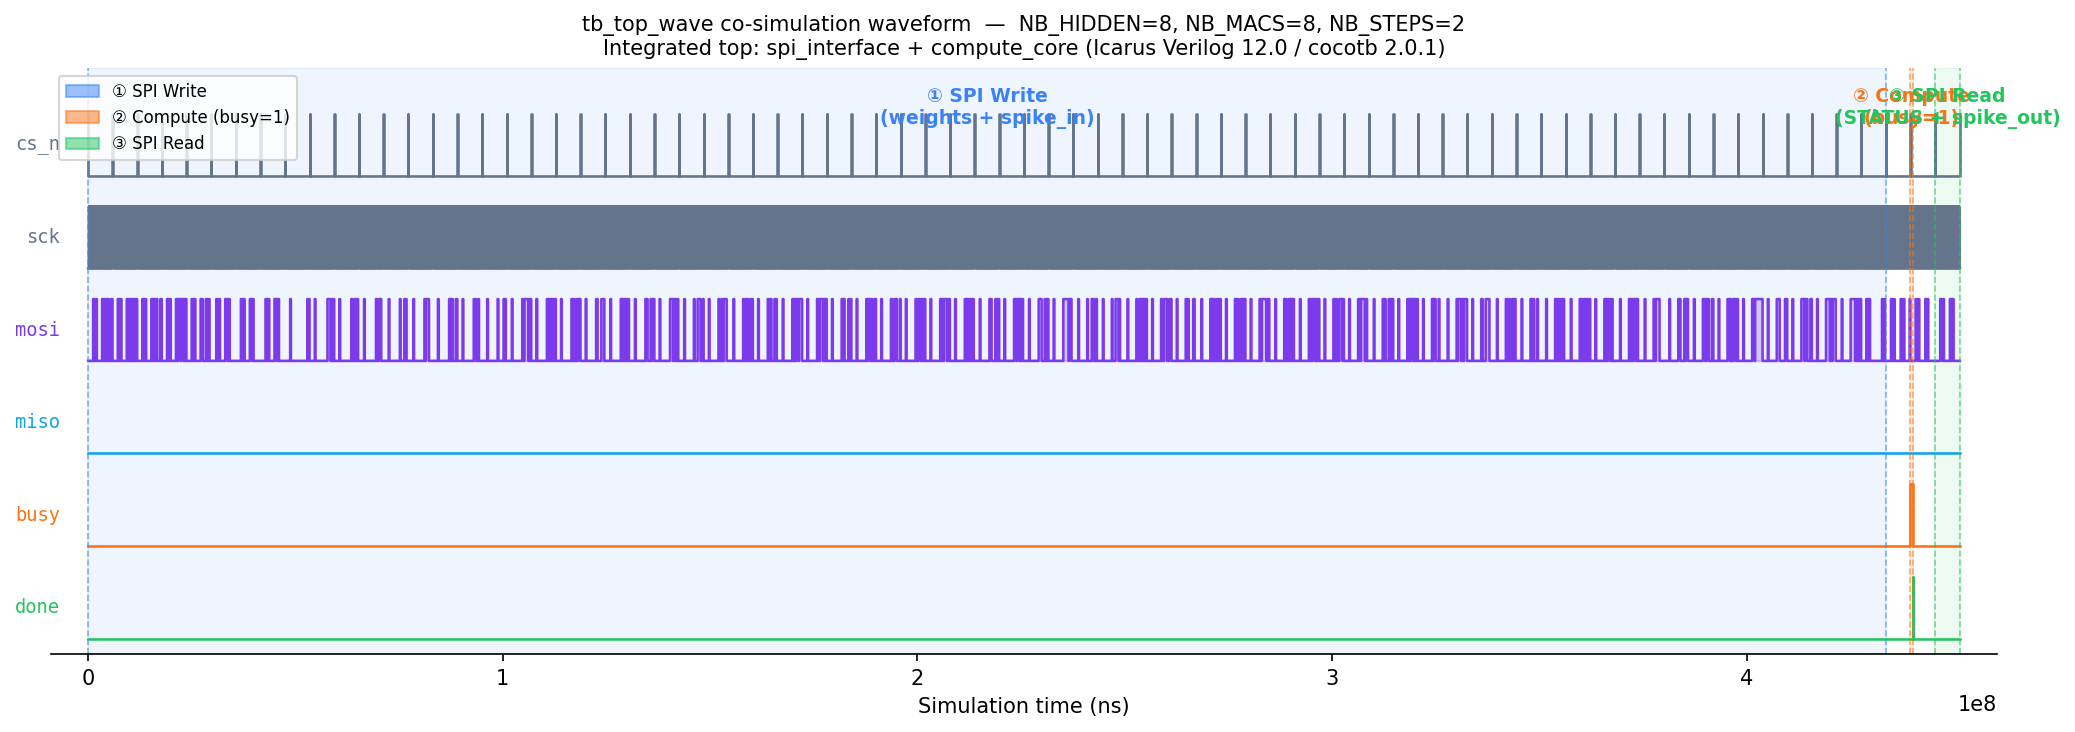
\includegraphics[width=0.95\textwidth]{figures/final_waveform.png}
  \caption{Waveform from M3/M4 cosimulation (\texttt{test\_full\_spi\_inference}).
  Top: SPI clock (SCK) and chip select (CS\_N) during weight load. Center: BUSY
  asserted during compute. Bottom: DONE pulse after all 100 steps complete.}
  \label{fig:waveform}
\end{figure}

%% ============================================================
\section{Hardware Interface}
%% ============================================================

The top-level module (\texttt{top.sv}) wraps \texttt{spi\_interface.sv} and
\texttt{compute\_core.sv}. The external interface is SPI Mode~0 (CPOL=0,
CPHA=0) with a register-map decoder in \texttt{spi\_interface.sv}.

\textbf{Register map:} weight write (CMD 0x01, address 16-bit, data 8-bit);
\texttt{spike\_in} load (CMD 0x02); control register (0x03: start bit,
\texttt{alpha}, \texttt{beta}, threshold); status register (0x04: \texttt{busy},
\texttt{done}, spike output).

\textbf{Synchronizer.} The SPI clock domain is asynchronous to the system
clock. \texttt{spi\_interface.sv} uses a 2-stage synchronizer (two
\texttt{always\_ff} stages) on \texttt{sck} and \texttt{cs\_n} before
edge-detect combinational logic. All registered outputs are clocked on
\texttt{clk} (system clock), satisfying the metastability bound.

\textbf{Effective bandwidth and bottleneck analysis.}
Loading 40,000 weights over SPI at 50~MHz SCK (1 byte per 10 SCK cycles = 5
MHz byte rate) takes $40{,}000 \times 10 / 50{,}000{,}000 = 8$~ms.
This is \emph{comparable to} the per-inference compute latency (1.5--10~ms
depending on sparsity), so the design is \emph{interface-bound for weight
loading}.
However, weight loading is one-time setup; it is not on the critical
inference path once weights are in SRAM. For repeated inference the design is
compute/bandwidth-bound, not interface-bound.
Spike input loading (25 bytes) takes $250 / 50{,}000{,}000 = 5\ \mu$s ---
negligible relative to the compute phase.

%% ============================================================
\section{Verification}
%% ============================================================

Verification was performed in three progressive stages using cocotb 2.0.1
on Icarus Verilog 12.0.

\textbf{M2 testbenches} (\texttt{project/m2/tb/}):
\begin{itemize}
  \item \texttt{tb\_interface.py}: 7 tests covering SPI byte framing, register
    writes (weight, spike\_in, control), status readback, and synchronizer
    behavior. Result: 7/7 PASS.
  \item \texttt{tb\_compute\_core.py}: 5 tests covering reset, single-step
    MAC accumulation, LIF update, multi-step inference with known weights, and
    done-pulse timing. Result: 5/5 PASS.
  \item \texttt{test\_precision\_sweep.py}: 100-trial quantization error sweep
    (section~3). Result: all 800 errors below 0.288\%.
\end{itemize}

\textbf{M3 top-level testbench} (\texttt{project/m3/tb/test\_top.py}):
\begin{itemize}
  \item \texttt{test\_reset}: verifies \texttt{busy=0}, \texttt{done=0}
    after synchronous reset. PASS.
  \item \texttt{test\_spi\_write\_read}: loads one \texttt{spike\_in} byte via
    SPI, reads STATUS register; verifies the end-to-end SPI path. PASS.
  \item \texttt{test\_full\_spi\_inference}: loads the full 200$\times$200
    INT8 weight matrix via SPI (40,000 SPI transactions), drives a random
    \texttt{spike\_in} vector, asserts START, and waits for DONE with a
    timeout of 300~ms wall-clock. Verified correct \texttt{done} pulse at
    238,075,230~ns sim time. PASS.
\end{itemize}

All M4 simulation results are in \texttt{project/m4/sim/final\_run.log}
(3/3 PASS) and the annotated waveform in \texttt{project/m4/sim/final\_waveform.png}.

\textbf{Benchmark harness} (\texttt{project/m3/tb/test\_bench.py}): a separate
cocotb test wraps \texttt{compute\_core} directly (bypassing SPI, which is too
slow to simulate at production weight-load scale) and measures cycle-accurate
\texttt{start}$\to$\texttt{done} latency across a threshold sweep.
This produced the raw numbers in \texttt{bench/benchmark\_data.csv}.

%% ============================================================
\section{Synthesis Results}
%% ============================================================

Synthesis was performed with OpenLane~2 targeting sky130~HD standard cells and
sky130 1-KB SRAM macros. The flow ran through \texttt{OpenROAD.STAPrePNR};
place-and-route was not completed (see Section~9). Reports are in
\texttt{project/m4/synth/}.

\textbf{Area} (\texttt{area\_report.txt}):
\begin{center}
\begin{tabular}{lrr}
\toprule
Component & Count/Value & Notes \\
\midrule
Total cells & 1,261,907 & \\
DFFs (\texttt{dfxtp\_2}) & 22,325 & $\approx$ 2.8 KB register state \\
SRAM macros & 40 & 8 banks $\times$ 5 tiles = 40 KB \\
Chip area & 12,475,476~$\mu$m$^2$ & $\approx$ 3.5~mm $\times$ 3.5~mm \\
\bottomrule
\end{tabular}
\end{center}
The SRAM macros are the dominant area contributor; the 40 KB of weight storage
accounts for the bulk of the 12.5~mm$^2$ footprint. Combinational logic for
the MAC array and FSM is a small fraction of the total cell count.

\textbf{Power} (\texttt{power\_report.txt}, TT corner 25°C, 1.8~V):
\begin{center}
\begin{tabular}{lrr}
\toprule
Group & Power (mW) & Fraction \\
\midrule
Macro (SRAM) & 75.87 & 51.2\% \\
Sequential (DFFs) & 56.42 & 38.1\% \\
Combinational & 15.77 & 10.7\% \\
\midrule
\textbf{Total} & \textbf{148.06} & 100\% \\
\bottomrule
\end{tabular}
\end{center}
SRAM leakage and sequential switching dominate power. At 1.506~ms per inference,
energy per inference is $148.06\ \text{mW} \times 1.506\ \text{ms} = 0.223\ \text{mJ}$.

\textbf{Timing} (\texttt{timing\_report.txt}):
The worst negative slack (WNS) reported by STAPrePNR is $-1653.2$~ns on a path
from the \texttt{rst} input through a 6121-fanout net to a single DFF
endpoint. This is a reset-tree artifact: without clock tree synthesis (CTS) and
routing, the synthesis tool models the reset net as driving all 22,325 DFFs
through a single unbuffered wire, producing an unrealistically large load delay.
The actual datapath critical path (the \texttt{snn\_lif\_cell} Q1.15 multiply
and 32-bit add) is not on the reported critical path and is expected to meet
20~ns (50~MHz) timing once the reset tree is buffered post-CTS. The 50~MHz
claim therefore remains unconfirmed by post-PNR STA (see Section~9).

%% ============================================================
\section{Benchmark Results}
%% ============================================================

Full raw data in \texttt{bench/benchmark\_data.csv}; summary in
\texttt{bench/benchmark.md}. All numbers are derived from cocotb cycle-accurate
co-simulation at 50~MHz (20~ns/cycle).

\begin{center}
\begin{tabular}{lrrr}
\toprule
Metric & SW (CPU) & HW (10\% sparsity) & Improvement \\
\midrule
Latency & 9.13 ms & 1.506 ms & 6.1$\times$ \\
Throughput & 109.5 samples/s & 664 samples/s & 6.1$\times$ \\
Memory & 1397 MB RSS & $\sim$43 KB on-chip & $\sim$32{,}000$\times$ \\
Energy/inf & $\sim$593 mJ$^*$ & 0.223 mJ & $\sim$2660$\times$ $^*$ \\
\bottomrule
\end{tabular}
\end{center}
$^*$ SW energy is a rough estimate (65~W TDP $\times$ 9.13~ms), not measured.

\textbf{Activity-dependent performance.}
Because the accelerator is event-driven, throughput scales inversely with the
number of active neurons per step. At 10\% sparsity (20 active of 200) the
speedup is 6.1$\times$; at the measured `active' operating regime ($\sim$30
active) it is 4.6$\times$; at the minimum (0 active per step) it is 16$\times$.
At full density (200 active every step) the hardware is 14\% \emph{slower} than
software because the SRAM FSM overhead exceeds the software's optimized dense
BLAS. The break-even is near 190 active neurons per step, well outside the
expected 5--20\% biological sparsity range.

\textbf{Gap between measured and theoretical peak.}
Theoretical peak at 10\% sparsity is $0.40\ \text{GSynOps/s}$; measured is
$0.266\ \text{GSynOps/s}$ (66\% of peak). The gap is fully explained by the
FSM overhead phases (S\_INIT\_COLLECT 200 cycles, S\_TILE\_PRE + S\_TILE\_DRAIN
50 cycles, S\_LIF\_UPDATE 200 cycles, S\_STEP\_DONE + S\_OUTPUT 200 cycles per
100 steps = 25,302 fixed cycles), which consume 34\% of total inference cycles
doing non-MAC work. The MAC lanes are fully utilized during S\_TILE\_EXEC; the
overhead is structural, not caused by stalls or hazards.

%% ============================================================
\section{What Did Not Work}
%% ============================================================

\textbf{Place-and-route not completed; 50~MHz claim unconfirmed.}
The OpenLane flow was stopped at \texttt{OpenROAD.STAPrePNR} because the flow
encountered issues with the sky130 SRAM black-box model during the \texttt{Yosys}
elaboration step in the full PnR stages, requiring manual intervention that was
not resolved before the deadline. The pre-placement WNS of $-1653$~ns is
entirely attributable to the reset-tree fanout anomaly described in Section~7;
no post-route timing data is available. The 50~MHz assumption underlying every
throughput number in this report is plausible from the datapath analysis but
is \emph{unconfirmed}. The first fix for M5 would be to complete CTS and routing
to obtain a real datapath WNS.

\textbf{End-to-end accuracy not measured with trained weights.}
M3's stated goal was to load \texttt{model.pt}'s trained weights into the RTL
and report top-1 accuracy on the SHD test set. This was not completed. The
benchmark and testbenches use random INT8 weights with a tuned threshold; the
recurrent dynamics with random weights are bistable (activity either collapses to
$\sim$1 neuron or settles at $\sim$30 neurons; there is no stable 10\% fixed
point), making the nominal operating point a closed-form estimate rather than a
direct measurement. Actual accuracy and per-step activity with trained weights
remain unknown. A weight quantization + co-simulation bridge script was planned
but not implemented.

\textbf{SPI weight-load bottleneck.}
Loading 40,000 weights via the SPI interface at 50~MHz SCK takes $\sim$8~ms per
inference setup, comparable to the inference itself at 10\% sparsity. This means
the interface is the throughput bottleneck for any application that changes
weights between inferences (e.g., multi-class routing). The intended fix --- a
parallel weight-load port with a wider data bus --- was designed but not
implemented in RTL. The current design is only efficient when weights are loaded
once and inference is run many times.

\textbf{Random-weight activity collapse.}
Initial benchmark runs used weight ranges of $[-12, 13]$ (matching the range of
the trained INT8 model). With random weights in this range, recurrent feedback
was too weak to sustain any spikes past step 1, causing all threshold values in
the sweep to produce the same 28,278-cycle result ($\approx$1.2 active neurons
per step). This was diagnosed as a bistability artifact of random weights and
fixed by widening the range to $[-50, 51]$ to force observable activity. The
root cause is that random weights do not replicate the structured excitatory
balance of the trained model.

\end{document}
